% ============================================================
% 第11章：ε-N 语言——极限的严格定义
% ============================================================

\chapter{ε-N 语言——极限的严格定义}

\begin{applicationbox}
\textbf{学完本章你能做什么？}
\begin{enumerate}
  \item 用 \textbf{ε-N 语言} 精确地定义"极限"——不再依赖直觉
  \item 用 ε-N 证明简单的极限（如 \(\dfrac{1}{n} \to 0\)）
  \item 掌握收敛数列的性质：唯一性、有界性、保号性
  \item 学会极限的四则运算法则
\end{enumerate}
\end{applicationbox}


% ============================================================
\section{从第10章来——从"趋近"到"精确"}
% ============================================================

第10章我们说"\(\lim a_n = L\) 意思是 \(a_n\) 越来越接近 \(L\)"。

但什么叫"越来越接近"？多近才算"足够近"？

数学家的回答是：

\begin{quote}
\textbf{不管你要多近（多小的 \(\varepsilon\)），我都能找到一项 \(N\)，使得 \(N\) 之后的所有项都在这个范围内。}
\end{quote}

这就是 ε-N 语言的核心思想。它把"无限趋近"这个模糊的概念，变成了\textbf{一个关于 \(\varepsilon\) 和 \(N\) 的精确陈述}。


% ============================================================
\section{ε-N 定义}
% ============================================================

\begin{definitionbox}[数列极限的 ε-N 定义]
设 \(\{a_n\}\) 是一个数列，\(L\) 是一个实数。

如果对\textbf{任意}给定的 \(\varepsilon > 0\)，都\textbf{存在}一个正整数 \(N\)，
使得当 \(n > N\) 时，有
\[
|a_n - L| < \varepsilon
\]
则称 \(\{a_n\}\) \textbf{收敛}于 \(L\)，记作 \(\displaystyle \lim_{n \to \infty} a_n = L\)。

如果不存在这样的 \(L\)，则称 \(\{a_n\}\) \textbf{发散}。
\end{definitionbox}

\begin{examplebox}[1——把定义"翻译"成中文]
\[
\lim_{n \to \infty} \frac{1}{n} = 0
\]

ε-N 语言翻译：

\begin{center}
\fcolorbox{green!30}{green!5}{\parbox{0.85\textwidth}{
\textbf{任给你一个正数 \(\varepsilon\)（不管多小），}\\
\textbf{我都能找到一个 \(N\)，使得从第 \(N+1\) 项开始，}\\
\textbf{所有 \(\dfrac{1}{n}\) 与 0 的差都小于 \(\varepsilon\)。}
}}
\end{center}

\textbf{举个例子：}
\begin{itemize}
  \item 取 \(\varepsilon = 0.1\)：要求 \(|\frac{1}{n} - 0| < 0.1\)，即 \(\frac{1}{n} < 0.1\)，\(n > 10\)。取 \(N = 10\)。
  \item 取 \(\varepsilon = 0.01\)：要求 \(\frac{1}{n} < 0.01\)，\(n > 100\)。取 \(N = 100\)。
  \item 取 \(\varepsilon = 0.001\)：要求 \(\frac{1}{n} < 0.001\)，\(n > 1000\)。取 \(N = 1000\)。
\end{itemize}

\(\varepsilon\) 越小，需要的 \(N\) 越大——但\textbf{总能找到}。
\end{examplebox}


% ============================================================
\section{用 ε-N 证明极限}
% ============================================================

\begin{examplebox}[2——证明 1/n 趋于 0]
\textbf{证明：}

对任意 \(\varepsilon > 0\)，我们要找 \(N\) 使得 \(n > N\) 时 \(|\frac{1}{n} - 0| < \varepsilon\)。

\[
\left|\frac{1}{n} - 0\right| = \frac{1}{n} < \varepsilon \;\Longleftrightarrow\; n > \frac{1}{\varepsilon}
\]

所以取 \(N = \left\lceil \frac{1}{\varepsilon} \right\rceil\)（\(\lceil\cdot\rceil\) 是向上取整），
则当 \(n > N\) 时，\(n > \frac{1}{\varepsilon}\)，从而 \(\frac{1}{n} < \varepsilon\)。

所以 \(\displaystyle \lim_{n\to\infty} \frac{1}{n} = 0\quad\blacksquare\)

\textbf{验证：} 若 \(\varepsilon = 0.01\)，则 \(N = \lceil 1/0.01 \rceil = 100\)。\\
当 \(n = 101\) 时，\(1/101 \approx 0.0099 < 0.01\) [OK]
\end{examplebox}

\begin{examplebox}[3——证明 n/(2n+1) 趋于 1/2]
\textbf{分析：}
\[
\left|\frac{n}{2n+1} - \frac{1}{2}\right|
= \left|\frac{2n - (2n+1)}{2(2n+1)}\right|
= \left|\frac{-1}{2(2n+1)}\right|
= \frac{1}{2(2n+1)} < \frac{1}{4n}
\]

\textbf{证明：} 对任意 \(\varepsilon > 0\)，要 \(\frac{1}{2(2n+1)} < \varepsilon\)。

由 \(\frac{1}{2(2n+1)} < \frac{1}{4n}\)，只需 \(\frac{1}{4n} < \varepsilon\)，即 \(n > \frac{1}{4\varepsilon}\)。

取 \(N = \left\lceil \frac{1}{4\varepsilon} \right\rceil\)，则当 \(n > N\) 时：
\[
\left|\frac{n}{2n+1} - \frac{1}{2}\right| = \frac{1}{2(2n+1)} < \frac{1}{4n} < \varepsilon
\]

所以 \(\displaystyle \lim_{n\to\infty} \frac{n}{2n+1} = \frac{1}{2}\quad\blacksquare\)
\end{examplebox}

\begin{examplebox}[4——证明 1/2的n次方 趋于 0]
\textbf{分析：} 要 \(\frac{1}{2^n} < \varepsilon\)，即 \(2^n > \frac{1}{\varepsilon}\)。

两边取对数：\(n \ln 2 > \ln\frac{1}{\varepsilon}\)，即 \(n > \frac{\ln(1/\varepsilon)}{\ln 2}\)。

\textbf{证明：} 对任意 \(\varepsilon > 0\)，取 \(N = \left\lceil \frac{\ln(1/\varepsilon)}{\ln 2} \right\rceil\)，
则当 \(n > N\) 时，\(2^n > 2^N \ge \frac{1}{\varepsilon}\)，从而 \(\frac{1}{2^n} < \varepsilon\)。

所以 \(\displaystyle \lim_{n\to\infty} \frac{1}{2^n} = 0\quad\blacksquare\)

\textbf{验证：} 取 \(\varepsilon = 0.001\)，则 \(N = \lceil \ln(1000)/\ln 2 \rceil = \lceil 6.91/0.693 \rceil = \lceil 9.97 \rceil = 10\)。\\
当 \(n=10\) 时，\(1/2^{10} = 1/1024 \approx 0.00098 < 0.001\) [OK]
\end{examplebox}


% ============================================================
\section{ε-N 的几何意义}
% ============================================================

\begin{examplebox}[5——ε 越小，N 越大]
\begin{center}
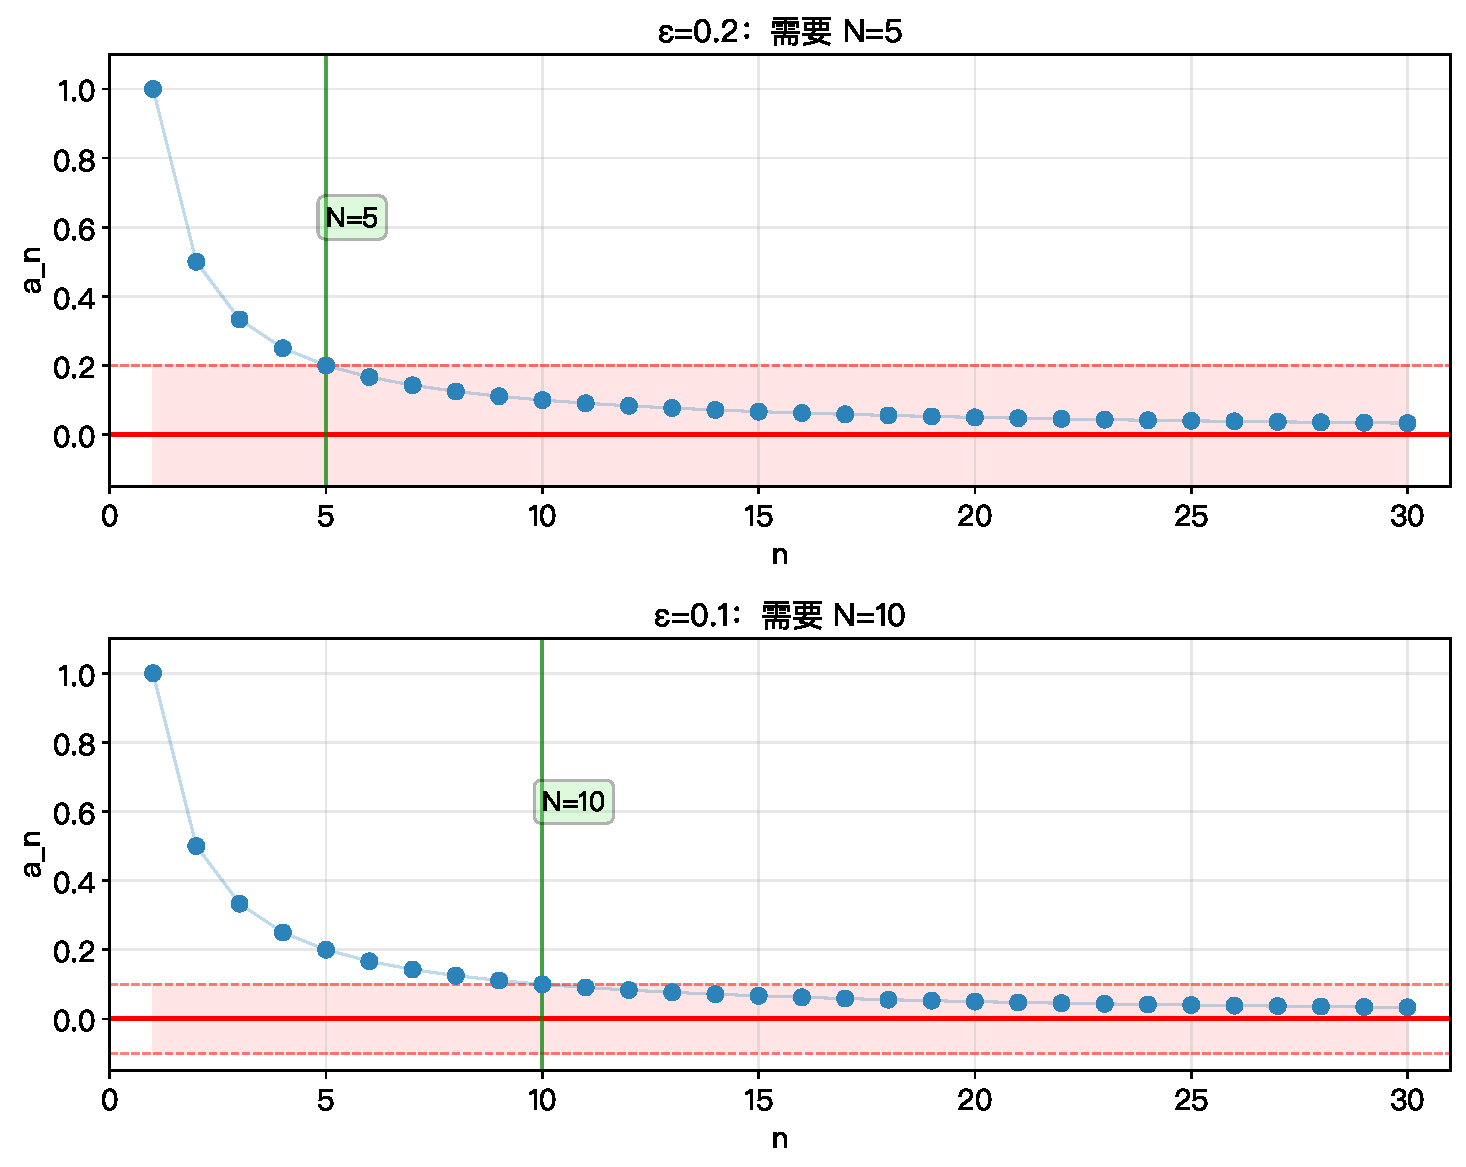
\includegraphics[width=0.85\textwidth]{figures/ch11_epsilon_N_demo.pdf}
\end{center}

\textbf{上图：} \(\varepsilon = 0.2\)，需要 \(N = 5\)（从第 6 项开始都在带内）\\
\textbf{下图：} \(\varepsilon = 0.1\)，需要 \(N = 10\)（从第 11 项开始都在带内）

\(\varepsilon\) 越小——要求越精确——需要等待的项数 \(N\) 就越大。
但\textbf{不管多小的 \(\varepsilon\)，总存在有限的 \(N\)}——这就是极限的本质。
\end{examplebox}


% ============================================================
\section{收敛数列的基本性质}
% ============================================================

\begin{theorembox}[极限的唯一性]
如果 \(\displaystyle\lim_{n\to\infty} a_n = L\) 且 \(\displaystyle\lim_{n\to\infty} a_n = M\)，则 \(L = M\)。

\textbf{解释：} 一个数列不能收敛到两个不同的数。极限如果存在，必定唯一。
\end{theorembox}

\begin{theorembox}[收敛数列必有界]
如果 \(\displaystyle\lim_{n\to\infty} a_n = L\)，则存在 \(M > 0\) 使得 \(|a_n| \le M\) 对所有 \(n\) 成立。

\textbf{解释：} 收敛的数列一定是有界的（但不一定单调）。
反过来不对——有界不一定收敛（如 \((-1)^n\) 有界但不收敛）。
\end{theorembox}

\begin{theorembox}[极限的保号性]
如果 \(\displaystyle\lim_{n\to\infty} a_n = L > 0\)，则存在 \(N\) 使得 \(n > N\) 时 \(a_n > 0\)。

\textbf{解释：} 如果极限是正数，那么足够靠后的项也都是正数。
\end{theorembox}


% ============================================================
\section{极限的四则运算}
% ============================================================

\begin{theorembox}[极限的四则运算法则]
如果 \(\displaystyle\lim_{n\to\infty} a_n = A\)，\(\displaystyle\lim_{n\to\infty} b_n = B\)，则：
\begin{align*}
  \lim_{n\to\infty} (a_n \pm b_n) &= A \pm B \\
  \lim_{n\to\infty} (a_n \cdot b_n) &= A \cdot B \\
  \lim_{n\to\infty} \frac{a_n}{b_n} &= \frac{A}{B} \quad (B \neq 0)
\end{align*}
\end{theorembox}

\begin{examplebox}[6——用四则运算法则求极限]
\[
\lim_{n\to\infty} \frac{3n^2 + 2n - 1}{2n^2 + 5}
\]

分子分母同除以 \(n^2\)：
\[
\frac{3n^2 + 2n - 1}{2n^2 + 5} = \frac{3 + \frac{2}{n} - \frac{1}{n^2}}{2 + \frac{5}{n^2}}
\]

因为 \(\frac{1}{n} \to 0\)，\(\frac{1}{n^2} \to 0\)，所以：
\[
\lim_{n\to\infty} \frac{3n^2 + 2n - 1}{2n^2 + 5} = \frac{3 + 0 - 0}{2 + 0} = \frac{3}{2}
\]

\textbf{口诀：} 分子分母同除以最高次项，低次项在 \(n\to\infty\) 时趋于 0。
\end{examplebox}


% ============================================================
\section{符号卡片}
% ============================================================

\begin{symbolcard}
\(\varepsilon\) & \verb|\varepsilon| & 读作"伊普西龙" & 任意小的正数 \\
\(N\) & —— & 读作"N" & 正整数，保证 \(n>N\) 时成立 \\
\(\lceil x \rceil\) & \verb|\lceil x\rceil| & 读作"x 的上取整" & 不小于 \(x\) 的最小整数 \\
\(|a_n-L|<\varepsilon\) & —— & 读作"epsilon" & 与极限的距离小于 epsilon \\
\end{symbolcard}


% ============================================================
\section{本章小结}
% ============================================================

\begin{progressbox}
\textbf{ε-N 定义}：\(\forall \varepsilon > 0, \exists N, n > N \Rightarrow |a_n - L| < \varepsilon\)

\textbf{证明步骤}：
\begin{enumerate}
  \item 从 \(|a_n - L|\) 出发，用不等式放大到关于 \(n\) 的简单形式
  \item 令其 \(< \varepsilon\)，解出 \(n\) 需要满足的条件
  \item 取 \(N\) 为这个条件的上取整
\end{enumerate}

\textbf{收敛数列性质}：极限唯一、收敛必有界、保号性

极限的四则运算法则：和的极限 = 极限的和，积的极限 = 极限的积，商的极限 = 极限的商
\end{progressbox}

\subsection*{通往下一章}

\textbf{这一章}你掌握了极限的严格定义和基本性质。

\textbf{下一章}我们学习判断极限存在的两大工具——
\textbf{单调有界原理}和\textbf{夹逼定理}（迫敛性）。
你会看到如何在不直接求极限的情况下，判断极限是否存在并求出它的值。


% ============================================================
% 习题
% ============================================================
\section{习题}

% ===== 送分 =====

\begin{exercise}[0]
用 ε-N 语言写出 "\(\lim a_n = 3\)" 的定义。
\end{exercise}

\begin{exercise}[0]
如果对 \(\varepsilon = 0.1\) 找到 \(N = 50\)，那么 \(n = 100\) 时 \(|a_n - L|\) 一定小于 0.1 吗？
\end{exercise}

\begin{exercise}[0]
数列极限存在，则极限必\_\_\_\_（唯一/不唯一）。
\end{exercise}

\begin{exercise}[0]
若 \(a_n \to 2\)，则 \(2a_n \to\) \_\_\_\_。
\end{exercise}

% ===== 简单 =====

\begin{exercise}[1]
用 ε-N 语言证明 \(\displaystyle \lim_{n\to\infty} \frac{1}{n^2} = 0\)。
\end{exercise}

\begin{exercise}[1]
若 \(\varepsilon = 0.01\)，对于 \(\frac{1}{n} \to 0\)，对应的 \(N\) 至少是多少？
\end{exercise}

\begin{exercise}[1]
判断对错：若数列有界，则一定收敛。
\end{exercise}

\begin{exercise}[1]
求极限：
\[
\lim_{n\to\infty} \frac{n+2}{n+1}
\]
\end{exercise}

% ===== 基础 =====

\begin{exercise}[2]
用 ε-N 语言证明 \(\displaystyle \lim_{n\to\infty} \frac{1}{\sqrt{n}} = 0\)。
\end{exercise}

\begin{exercise}[2]
已知 \(a_n \to 3\)，用四则运算法则求：
\[
\lim_{n\to\infty} (2a_n + 1),\quad \lim_{n\to\infty} \frac{a_n}{a_n + 1}
\]
\end{exercise}

\begin{exercise}[2]
若 \(\displaystyle \lim_{n\to\infty} a_n = L\)，证明 \(\displaystyle \lim_{n\to\infty} (a_n)^2 = L^2\)。
（提示：\(|a_n^2 - L^2| = |a_n - L| \cdot |a_n + L|\)，再说明 \(|a_n + L|\) 有界）
\end{exercise}

\begin{exercise}[2]
求极限：
\[
\lim_{n\to\infty} \frac{2n^2 - 3n + 1}{5n^2 + 4n - 2}
\]
\end{exercise}

% ===== 普通 =====

\begin{exercise}[3]
用 ε-N 语言证明 \(\displaystyle \lim_{n\to\infty} \frac{2n}{n+3} = 2\)。
\end{exercise}

\begin{exercise}[3]
求极限：
\[
\lim_{n\to\infty} \frac{n^3 + 2n}{2n^3 - n^2 + 1}
\]
\end{exercise}

\begin{exercise}[3]
已知 \(a_n \to A\)，\(b_n \to B\)，证明 \(a_n b_n \to AB\)。
\end{exercise}

\begin{exercise}[3]
若 \(a_n \to 0\)，\(b_n\) 有界，证明 \(a_n b_n \to 0\)。
\end{exercise}

\begin{exercise}[3]
用 ε-N 语言证明：若 \(a_n \to L\)，则 \(|a_n| \to |L|\)。
\end{exercise}

% ===== 中等 =====

\begin{exercise}[4]
求极限：
\[
\lim_{n\to\infty} (\sqrt{n+1} - \sqrt{n})
\]
（提示：有理化 \(\sqrt{n+1} - \sqrt{n} = \frac{1}{\sqrt{n+1} + \sqrt{n}}\)）
\end{exercise}

\begin{exercise}[4]
用 ε-N 语言证明 \(\displaystyle \lim_{n\to\infty} \frac{n^2}{n^2 + 1} = 1\)。
\end{exercise}

\begin{exercise}[4]
已知 \(a_1 = 1\)，\(a_{n+1} = \frac{a_n + 2}{2}\)。
\begin{enumerate}
  \item[(1)] 写出前 5 项，观察规律
  \item[(2)] 求极限（设极限为 \(L\)，在递推式两边取极限）
\end{enumerate}
\end{exercise}

\begin{exercise}[4]
求极限：
\[
\lim_{n\to\infty} \frac{1 + 2 + 3 + \cdots + n}{n^2}
\]
\end{exercise}

\begin{exercise}[4]
证明：收敛数列必有界。
（提示：取 \(\varepsilon = 1\)，则存在 \(N\) 使 \(n>N\) 时 \(|a_n - L| < 1\)，
然后前 \(N\) 项有限，后 \(N\) 项有界）
\end{exercise}

% ===== 进阶 =====

\begin{exercise}[5]
用 ε-N 语言证明 \(\displaystyle \lim_{n\to\infty} \frac{\sin n}{n} = 0\)。
（提示：\(|\sin n| \le 1\)）
\end{exercise}

\begin{exercise}[5]
已知 \(a_n \to L\)，用 ε-N 语言证明 \(a_{n+1} \to L\)。
\end{exercise}

\begin{exercise}[5]
求极限：
\[
\lim_{n\to\infty} \frac{n^2 + (-1)^n n}{n^2 + 1}
\]
\end{exercise}

\begin{exercise}[5]
已知 \(a_1 = \sqrt{2}\)，\(a_{n+1} = \sqrt{2 + a_n}\)。
\begin{enumerate}
  \item[(1)] 写出前 3 项
  \item[(2)] 若极限存在，求它的值
\end{enumerate}
\end{exercise}

% ===== 拔高 =====

\begin{exercise}[6]
设 \(a_n = \frac{n^k}{2^n}\)（\(k\) 是正整数）。
试说明为什么 \(\displaystyle \lim_{n\to\infty} a_n = 0\)。
（提示：指数 \(2^n\) 的增长最终会超过任何幂函数 \(n^k\)）
\end{exercise}

\begin{exercise}[6]
用 ε-N 语言证明 \(\displaystyle \lim_{n\to\infty} \frac{2^n}{n!} = 0\)。
（提示：\(n \ge 4\) 时 \(\frac{2^n}{n!} \le \frac{2}{n}\)）
\end{exercise}

\begin{exercise}[6]
已知 \(a_n \to L\)，定义 \(b_n = \frac{a_1 + a_2 + \cdots + a_n}{n}\)（算术平均）。
证明 \(b_n \to L\)。
（提示：把前 \(N\) 项和后 \(n-N\) 项分开处理）
\end{exercise}

% ===== 极难 =====

\begin{exercise}[7]
设 \(a_1 = 1\)，\(a_{n+1} = \frac{1}{2}\left(a_n + \frac{2}{a_n}\right)\)。
\begin{enumerate}
  \item[(1)] 证明 \(a_n^2 > 2\)（\(n \ge 2\)）
  \item[(2)] 证明 \(a_n\) 单调递减
  \item[(3)] 求 \(\displaystyle \lim_{n\to\infty} a_n\)
\end{enumerate}

\textbf{说明：} 这是牛顿法求 \(\sqrt{2}\) 的迭代序列。
先证有下界（\(a_n > \sqrt{2}\)），再证递减，最后两边取极限解出 \(L = \sqrt{2}\)。
这是数学分析中最经典的极限问题之一。
\end{exercise}
